\documentclass[12pt]{standalone}

\usepackage{tikz}
\usepackage{ctex}

\begin{document}
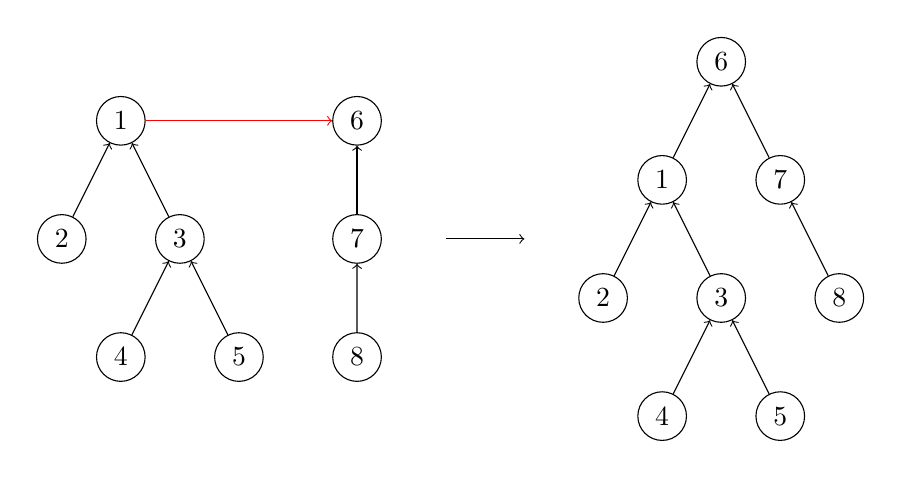
\begin{tikzpicture}

\matrix[column sep={3cm,between origins}] at (0,0)
{
    \scoped[<-,every node/.style={circle,draw}]
    \node (A) {1}
        child {node {2}}
        child {node {3}
            child {node {4}}
            child {node {5}}}; &
    \scoped[<-,every node/.style={circle,draw}]
    \node (B) {6} child {node {7} child {node {8}}}; \\
};

\draw[color=red,->] (A) -- (B);

\draw[->] (3,0) -- (4,0);

\matrix[column sep={3cm,between origins}] at (6.5,0)
{
    \scoped[<-,every node/.style={circle,draw}]
    \node {6}
        child {node {1}
            child {node {2}}
            child {node {3}
                child {node {4}}
                child {node {5}}}}
        child {node {7}
            child[missing]
            child {node {8}}}; \\
};

\end{tikzpicture}
\end{document}
